% !TeX root = er.tex

\chapter{Reactive Behavior}\label{ch.reactive}

\abstract*{The behavior of a robot is reactive if values returned by the sensors directly affect the actuators. Two families of reactive behavior are presented. Braitenberg vehicles are very simple robots that demonstrate relatively complex behavior. A robot with ground sensors can follow a line on a surface and thus navigate a known environment such as a warehouse. Three algorithms are presented: an algorithm that uses two ground sensors, an algorithm that uses only one ground sensor on a line with a gradient and an algorithm that follows the edge of a line.}

We are now ready to write our first algorithms for robots. These algorithms demonstrate \emph{reactive behavior}\index{reactive behavior}: an event (such as the detection of a nearby object by the robot) causes the robot to react by performing an action that changes its behavior (such as stopping the motors). Purely reactive behavior occurs when the action is related only to the occurrence of an event and does not depend on data stored in memory (state).

The reactive behaviors are those of \emph{Braitenberg vehicles} which are appropriate for introducing robotics because complex behavior arises from simple algorithms. Sections~\ref{s.braitenberg}--\ref{s.turning} describe Braitenberg vehicles that demonstrate reactive behavior; in Chapter~\ref{ch.fmg} we present Braitenberg vehicles that have non-reactive behavior with states. Section~\ref{s.line} presents several algorithms for the classic reactive behavior of line following. Line following is an interesting task because the algorithms are sensitive to the characteristics of the sensors and the lines. Calibration is necessary to determine the optimum thresholds for fast robust motion of the robot. Section~\ref{s.abstract-vehicles} gives a brief overview of Braitenberg's original formulation of the vehicles in a biological approach with sensors connected directly to the motors, not through a computer. Later in the book (Sect.~\ref{s.braitenberg-ann}) we discuss the implementation of Braitenberg vehicles using neural networks.


\section{Braitenberg vehicles}\label{s.braitenberg}
\index{Braitenberg vehicle}

Valentino Braitenberg was a neuroscientist who described the design of virtual vehicles that exhibited surprisingly complex behavior. Researchers at the MIT Media Lab developed hardware implementations of the vehicles from \emph{programmable bricks} that were the forerunner of the \lego{} Mindstorms robotics kits.\footnote{The MIT report uses the term \emph{Braitenberg creatures} but we retain the original term.} This chapter describes an implementation of most of the Braitenberg vehicles from the MIT report. The MIT hardware used light and touch sensors, while our generic robot is based upon horizontal proximity sensors.

To facilitate comparison with the MIT report (and indirectly with Braitenberg's book), the names of their vehicles have been retained, even though it may be difficult to understand their meanings in our implementations.

Two vehicles are presented in detail by giving all of the following:
\begin{itemize}
\item The specification of the behavior of the robot;
\item A formalized algorithm for the specified behavior;
\item An activity that asks you to implement the algorithm on your robot.
\end{itemize}
The other vehicles are presented in activities that specify the behavior and ask you to develop an algorithm and to implement it on your robot.

\section{Reacting to the detection of an object}\label{s.reacting}

\begin{quote}
\normalsize\noindent{}\textbf{Specification (Timid):}\index{Braitenberg vehicle!timid} When the robot does not detect an object, it moves forwards. When it detects an object, it stops.
\end{quote}
\noindent{}Algorithm~\ref{alg.timid} implements this behavior.

\begin{figure}
\begin{alg}{Timid}{timid}
\hline
\stl{}&when object not detected in front&\\
\stl{}&\idc{} left-motor-power \ass $100$&\\
\stl{}&\idc{} right-motor-power \ass $100$&\\
\stl{}&&\\
\stl{}&when object detected in front&\\
\stl{}&\idc{} left-motor-power \ass $0$&\\
\stl{}&\idc{} right-motor-power \ass $0$&\\
\end{alg}
\end{figure}

The algorithm uses two event handlers, one for the event of detecting an object and one for the event of not detecting an object. The event handlers are written using the \p{when} statement whose meaning is:

\begin{center}
\p{when the event \emph{first occurs}, perform the following actions}.
\end{center}
\noindent{}Why do we use this construct and not the more familiar \p{while} statement (Algorithm~\ref{alg.timid-a})?

\begin{figure}
\begin{alg}{Timid with while}{timid-a}
\hline
\stl{}&while object not detected in front&\\
\stl{}&\idc{} left-motor-power \ass $100$&\\
\stl{}&\idc{} right-motor-power \ass $100$&\\
\stl{}&&\\
\stl{}&while object detected in front&\\
\stl{}&\idc{} left-motor-power \ass $0$&\\
\stl{}&\idc{} right-motor-power \ass $0$&\\
\end{alg}
\end{figure}

If we use the \p{while} statement, \emph{as long as} the object is not detected the motors will be turned on, and \emph{as long as} the object is detected the motors will be turned off. Since the sensor will detect the object over a range of distances, the motors will be repeatedly turned on or off. It is likely that no harm will be done if a motor that is already off is turned off and a motor that is already on is turned on, but these repeated commands are not necessary and may waste resources. Therefore, we prefer to turn the motors off only when the object is first detected and to turn them on only when the object is first not detected. The \p{when} statement gives the semantics that we want.

\begin{framed}
\act{Timid}{timid}
\begin{itemize}
\item Implement the Timid behavior.
\end{itemize}
\end{framed}

\begin{framed}
\act{Indecisive}{indecisive}
\begin{itemize}
\item Implement the Indecisive behavior.
\begin{quote}
\normalsize\noindent\textbf{Specification (Indecisive):}\index{Braitenberg vehicle!indecisive} When the robot does not detect an object, it moves forwards. When it detects an object, it moves backwards.
\end{quote}
\item At just the right distance, the robot will \emph{oscillate}, that is, it will move forwards and backwards in quick succession. Measure this distance for your robot and for objects of different reflectivity.
\end{itemize}
\end{framed}

\begin{framed}
\act{Dogged}{dogged}
\begin{itemize}
\item Implement the Dogged behavior.
\begin{quote}
\normalsize\noindent\textbf{Specification (Dogged):}\index{Braitenberg vehicle!dogged} When the robot detects an object in front, it moves backwards. When the robot detects an object in back, it moves forwards.
\end{quote}
\end{itemize}
\end{framed}

\begin{framed}
\act{Dogged (stop)}{dogged1}
\begin{itemize}
\item Implement the Dogged (stop) behavior.
\begin{quote}
\normalsize\noindent\textbf{Specification (Dogged (stop)):}\index{Braitenberg vehicle!dogged} As in Activity~\ref{act.dogged}, but when an object is not detected, the robot stops.
\end{quote}
\end{itemize}
\end{framed}

\begin{framed}
\act{Attractive and repulsive}{attractive}
\begin{itemize}
\item Implement the Attractive and repulsive behavior.
\begin{quote}
\normalsize\noindent\textbf{Specification (Attractive and repulsive):}\index{Braitenberg vehicle!attractive and repulsive} When an object approaches the robot from behind, the robot runs away until it is out of range.
\end{quote}
\end{itemize}
\end{framed}

\section{Reacting and turning}\label{s.turning}

A car turns by changing the angle of its front wheels relative to the frame of the vehicle. The motor power is not changed. A robot with differential drive\index{differential drive!turning with} has no steering mechanism (like the steering wheel of a car or the handlebars of a bicycle). Instead, it turns by setting different levels of power to the left and right wheels. If one wheel turns faster than the other, the robot turns in the direction opposite that of the faster wheel  (Fig.~\ref{fig.left-gentle}). If one wheel turns backwards while the other turns forwards, the turn is much sharper (Fig.~\ref{fig.left-sharp}). In the figures, the arrows denote the direction and speed of each wheel. The \emph{turning radius}\index{turning radius} is the radius of the circle that is the path of the robot. We say that a turn is tighter if the radius is smaller. At the extreme, if one wheel turns forwards and the second turns backwards at the same speed, the robot will turn in place and the turning radius is zero.

\begin{figure}
\subfigures
\begin{minipage}{\textwidth}
\leftfigure[c]{
\begin{tikzpicture}
\pic[rotate=10,scale=1.2] at (0,0) { robot };
\draw[raxis] (0,0mm) -- (-80:15mm);
\draw[raxis] (0,0mm) -- (100:15mm);
\draw[raxis] (0,0) -- (10:8pt);
\draw[raxis] (0,0) -- (190:8pt);
\draw[->] (6mm,-8.5mm) -- +(10:15mm);
\draw[->] (3mm,10.3mm) -- +(10:5mm);
\end{tikzpicture}
}
\hspace{\fill}
\rightfigure[c]{
\begin{tikzpicture}
\pic[rotate=45,scale=1.2] at (0,0) { robot };
\draw[raxis] (0,0mm) -- (-45:15mm);
\draw[raxis] (0,0mm) -- (135:15mm);
\draw[raxis] (0,0) -- (45:8pt);
\draw[raxis] (0,0) -- (225:8pt);
\draw[->] (9.6mm,-3.6mm) -- +(45:15mm);
\draw[->] (-9.5mm,3.7mm) -- +(-135:5mm);
\end{tikzpicture}
}
\leftcaption{Gentle left turn\label{fig.left-gentle}}
\rightcaption{Sharp left turn\label{fig.left-sharp}}
\end{minipage}
\end{figure}

Let us now implement a Braitenberg vehicle whose specification requires the robot to turn.

\begin{quote}
\normalsize\noindent\textbf{Specification (Paranoid):}\index{Braitenberg vehicle!paranoid} When the robot detects an object, it moves forwards (colliding with the object). When it does not detect an object, it turns to the left.
\end{quote}
Algorithm~\ref{alg.paranoid} implements this behavior.

\medskip

\begin{alg}{Paranoid}{paranoid}
\hline
\stl{}&when object detected in front&\\
\stl{}&\idc{} left-motor-power \ass $100$&\\
\stl{}&\idc{} right-motor-power \ass $100$&\\
\stl{}&&\\
\stl{}&when object not detected in front&\\
\stl{}&\idc{} left-motor-power \ass $-50$&// Left motor backwards\\
\stl{}&\idc{} right-motor-power \ass $50$&// Right motor forwards\\
\end{alg}

\begin{framed}
\act{Paranoid}{paranoid}
\begin{itemize}
\item Implement the Paranoid behavior.
\item In the algorithm, the left and right motors are set to equal but opposite powers. Experiment with these power levels to see their influence on the turning radius of the robot.
\end{itemize}
\end{framed}

\begin{framed}
\act{Paranoid (right-left)}{paranoid1}
\begin{itemize}
\item Implement the Paranoid (right-left) behavior.
\begin{quote}
\normalsize\noindent\textbf{Specification (Paranoid (right-left)):}\index{Braitenberg vehicle!paranoid} When an object is detected in front of the robot, the robot moves forwards. When an object is detected to the right of the robot, the robot turns right. When an object is detected to the left of the robot, the robot turns left. When no object is detected the robot does not move.
\end{quote}
\end{itemize}
\end{framed}

\begin{framed}
\act{Insecure}{insecure}
\begin{itemize}
\item Implement the Insecure behavior.
\begin{quote}
\normalsize\noindent\textbf{Specification (Insecure):}\index{Braitenberg vehicle!insecure} If an object is not detected to the left of the robot, set the right motor to rotate forwards and set the left motor off. If an object is detected to the left of the robot, set the right motor off and set the left motor to rotate forwards.
\end{quote}
\item Experiment with the motor settings until the robot follows a wall to its left
\end{itemize}
\end{framed}

\begin{framed}
\act{Driven}{driven}
\begin{itemize}
\item Implement the Driven behavior.
\begin{quote}
\normalsize\noindent\textbf{Specification (Driven):}\index{Braitenberg vehicle!driven} If an object is detected to the left of the robot, set the right motor to rotate forwards and set the left motor off. If an object is detected to the right of the robot,  set the right motor off and set the left motor to rotate forwards.
\end{quote}
\item Experiment with the motor settings until the robot approaches the object in a zigzag.
\end{itemize}
\end{framed}


\section{Line Following}\label{s.line}
\index{line following}

Consider a warehouse with robotic carts that bring objects to a central dispatching area (Fig.~\ref{fig.warehouse}). Lines are painted on the floor of the warehouse and the robot is instructed to follow the lines until it reaches the storage bin of the desired object.

\begin{figure}
\begin{center}
\begin{tikzpicture}[thick, rounded corners, shelf/.style={draw, minimum height=1.2cm, rectangle split, rectangle split parts=2}]
\draw  (-.8,2.0) -- (-.8,1.7) -- (2.2,1.7) -- (2.2,0) -- (3.6,0) -- (3.6,1.7) -- (5.0,1.7) -- (5.0,0) -- (6.6,0) -- (6.6,2.8) -- (-.8,2.8) -- (-.8,2.6);
\node[draw, shape=rectangle, minimum height=1pt] at (-.8,2.3) {\textsf{Dispatch}};
\node[shelf] at (1.5,.8) {\textsf{A}\nodepart{two}\textsf{B}};
\node[shelf] at (2.9,.8) {\textsf{C}\nodepart{two}\textsf{D}};
\node[shelf] at (4.3,.8) {\textsf{E}\nodepart{two}\textsf{F}};
\node[shelf] at (5.7,.8) {\textsf{G}\nodepart{two}\textsf{H}};
\end{tikzpicture}
\caption{A robotic warehouse}\label{fig.warehouse}
\end{center}
\end{figure}

\emph{Line following} is a task that brings out all the uncertainty of constructing robots in the real world. The line might not be perfectly straight, dust may obscure part of the line, or dirt may cause one wheel to move more slowly than the other. To follow a line, the robot must decide whether it is on the line or not, and if it starts to leave the line on one side, it must turn in the correct direction to regain the line.

\subsection{Line following with a pair of ground sensors}

To follow a line, a pair of ground sensors can be used\index{sensor!ground} (Fig.~\ref{fig.ground-on-a-line}).\footnote{The figure shows a top view although the ground sensors are on the bottom of the robot.} A ground sensor on a light-colored floor will detect a lot of reflected light. If a dark line is painted on the floor, the sensor will detect very little reflected light when it is over the line.\footnote{Our presentation of the line following algorithms assumes that the floor is light-colored. If your floor is dark-colored, a white line should be used.} The line should be black for increased contrast with the white floor, but the figure displays the line in light gray so as not to obscure the robot and its sensors. Thresholds are used to determine when the event occurs of a sensor moving from detecting the line to detecting the floor or conversely.

\begin{figure}
\begin{center}
\begin{tikzpicture}[scale=1.1]
\draw[fill,lightgray] (-2,-3.5mm) rectangle +(7,8mm);
\pic at (0,0) { robot2 };
\end{tikzpicture}
\caption{A robot with two ground sensors over a line}\label{fig.ground-on-a-line}
\end{center}
\end{figure}

The line must be wide enough so that both ground sensors will sense dark when the robot is directly above the line. The sensors do not have to be entirely over the line; it is sufficient that the amount of light reflected from line onto the sensor be below the threshold defined for black.

To implement line-following, the robot must move forward whenever both sensors detect a dark surface, indicating that it is on the line. If the robot starts to leave the line, either the left or the right ground sensor will leave the line first (Fig.~\ref{fig.leave-left-right}):

\begin{figure}
\begin{center}
\begin{tikzpicture}[scale=1.1]
\draw[fill,lightgray] (-1,-3.5mm) rectangle +(7,8mm);
\pic[rotate=10] at (0,3mm) { robot2 };
\pic[rotate=-10] at (4,-3mm) { robot2 };
\end{tikzpicture}
\caption{Leaving the line\label{fig.leave-left-right}}
\end{center}
\end{figure}

\begin{itemize}
\item If the robot moves off the line to the \emph{left}, the \emph{left} sensor will not detect the line while the \emph{right} sensor is still detecting it; the robot must turn to the \emph{right}.
\item If the robot moves off the line to the \emph{right}, the \emph{right} sensor will not detect the line while the \emph{left} sensor is still detecting it; the robot must turn to the \emph{left}.
\end{itemize}
For now, we specify that the robot stops whenever neither sensor detects the line.

Algorithm~\ref{alg.line-two} formalizes the above informal description.

\begin{figure}
\begin{alg}{Line following with two sensors}{line-two}
\hline
\stl{}&when both sensors detect black&\\
\stl{}&\idc{} left-motor-power \ass $100$&\\
\stl{}&\idc{} right-motor-power \ass $100$&\\
\stl{}&&\\
\stl{}&when neither sensor detects black&\\
\stl{}&\idc{} left-motor-power \ass $0$&\\
\stl{}&\idc{} right-motor-power \ass $0$&\\
\stl{}&&\\
\stl{}&when only the left sensor detects black&\\
\stl{}&\idc{} left-motor-power \ass $0$&\\
\stl{}&\idc{} right-motor-power \ass $50$&\\
\stl{}&&\\
\stl{}&when only the right sensor detects black&\\
\stl{}&\idc{} left-motor-power \ass $50$&\\
\stl{}&\idc{} right-motor-power \ass $0$&\\
\end{alg}
\end{figure}

\begin{framed}
\act{Line following with two sensors}{line-following-one}
\begin{itemize}
\item Implement Algorithm~\ref{alg.line-two}.
\item Use black electrician's tape or gaffer tape to create a line on the floor. (Gaffer tape is used on stage and film sets to bind cables or fix them to the floor. Gaffer tape is usually less reflective than electrician's tape and thus a better choice for implementing line-following algorithms.)
\item The line should have angles or curves which will cause the robot to start running off the line. Run the program and check that the robot can successfully follow the line with its angles and curves.
\item Experiment with motor powers for turning back onto the line. If the turn is too gentle, the other sensor might also run off the line before the robot turns back. If the turn is too sharp, it might cause the robot to run off the other end of the line. In any case, sharp turns can be dangerous to the robot and cause whatever it is carrying to fall off.
\item The forward speed of the robot on the line is also important. If it is too fast, the robot can run off the line before the turning actions can affect its direction. If the speed is too slow, no one will buy your robot to use in a warehouse. How fast can your robot follow the line without running off it?
\end{itemize}
\end{framed}

\begin{framed}
\act{Different line configurations}{line-config}
\begin{itemize}
\item What is the sharpest turn that your robot can follow? Can it follow a line that has a $90^\circ$ turn?
\item Experiment with different configurations of the line: gentle turns, sharp turns and zigzag lines.
\item Experiment with the width of the line. What happens if the line is much wider or narrower than the distance between the sensors?
\end{itemize}
\end{framed}

\begin{framed}
\act{Regaining the line after losing it}{regaining}
\begin{itemize}
\item Modify the algorithm so that the robot returns to the line after it loses it, that is, when both sensors no longer detect black.
\item Algorithm 1: Before both sensors no longer detect the line, one of them will be the first that no longer detects the line. Use a variable to remember the sensor that first lost the line; when the line is lost, turn in the opposite direction of the value of this variable.
\item Algorithm 2: The previous algorithm might not work if the robot is moving too fast and runs off the line before it detects that only one sensor lost the line. Instead, if both sensors no longer detect black, cause the robot the search for the line for a short distance, first in one direction and then in the other direction.
\end{itemize}
\end{framed}

\begin{framed}
\act{Sensor configuration}{sensor-config}
\begin{itemize}
\item Discuss what effect the following modifications to the robot would have on its ability to follow a line:
\begin{itemize}
\item Ground sensing events occur more often or less often.
\item The sensors are further apart or closer together.
\item There are more than two ground sensors on the bottom of the robot.
\item The sensors are on the back of the robot or the robot moves backwards.
\end{itemize}
\item Experiment with these changes if they can be done on your robot.
\end{itemize}
\end{framed}

\subsection{Line following with only one ground sensor}

A robot can follow a line with only one ground sensor if the reflectivity of the line varies across its width. Figure~\ref{fig.gradient} shows a grayscale line whose shade varies continuously from fully black to fully white across its width. The ground sensor will return values from $0$ to $100$ depending on which part of the line it is over.

\begin{figure}
\begin{center}
\begin{tikzpicture}[scale=1.1]
\shadedraw[top color=black, bottom color = white] (-2,-3.5mm) rectangle +(7,8mm);
\pic at (0,0) { robot1 };
\end{tikzpicture}
\caption{A line with a grayscale gradient}\label{fig.gradient}
\end{center}
\end{figure}

When the robot is directly over the center of the line, the sensor will return the value $50$ that is midway between black and white. Of course, we don't expect the value to be exactly 50, so there is no reason for the robot to turn left or right unless the value approaches $0$ or $100$. We define two thresholds:
\begin{itemize}
\item \p{black-threshold}: below this value, the robot is leaving the left side of the line.
\item \p{white-threshold}: above this value, the robot is leaving the right side of the line.
\end{itemize}
Algorithm~\ref{alg.line-one} changes the motor power settings when the value returned by the sensor crosses the thresholds.

\begin{figure}
\begin{alg}{Line following with one sensor}{line-one}
&\idv{}integer black-threshold \ass 20&\\
&\idv{}integer white-threshold \ass 80&\\
\hline
\stl{}&when black-threshold $\leq$ sensor value $\leq$ white-threshold&\\
\stl{}&\idc{} left-motor-power \ass $100$&\\
\stl{}&\idc{} right-motor-power \ass $100$&\\
\stl{}&&\\
\stl{}&when sensor value $>$ white-threshold&\\
\stl{}&\idc{} left-motor-power \ass $-50$&\\
\stl{}&\idc{} right-motor-power \ass $50$&\\
\stl{}&&\\
\stl{}&when black-threshold $<$ sensor value&\\
\stl{}&\idc{} left-motor-power \ass $50$&\\
\stl{}&\idc{} right-motor-power \ass $-50$&\\
\end{alg}
\end{figure}

\begin{framed}
\act{Line following with one sensor}{line-following-two}
\begin{itemize}
\item Implement Algorithm~\ref{alg.line-one}.
\item Experiment with the thresholds until the robot can follow the line.
\item Modify the algorithm so that the robot detects when it has run completely off the line. Hint: The only problem is when the robot runs off the black side of the line, because there the algorithm doesn't distinguish between that case and running off the white side of the line. One solution is to use a variable to remember the previous value of the sensor, so that the two cases can be distinguished.
\end{itemize}
\end{framed}

\begin{framed}
\act{Line following with proportional correction}{line-following-proportional}
\begin{itemize}
\item Since the sensor values are proportional to the grayscale of the line, the approximate distance of the sensor from the center of the line can be computed. Modify the algorithm to compute this distance.
\item Modify the algorithm so that the motor setting is proportional to this distance.
\item Run experiments for various constants of proportion and explain the results.
\end{itemize}
\end{framed}

\subsection{Line following without a gradient}\label{s.no-gradient}

The receiver of a proximity sensor has an \emph{aperture}\index{apeture}, an opening through which the light is collected. Apertures are often wide in order to allow more light to fall on the sensor so that it will be responsive to low levels of light. Cameras have \emph{f-stops}: the lower the value of the f-stop, the wider the aperture, so pictures can be taken in relatively dark environments. If the aperture of the ground proximity sensor is relatively wide, a gradient on the line is not needed. A single sensor can follow one \emph{edge} of a line (Fig.~\ref{fig.no-gradient}). The figure assumes that the robot is supposed to follow the right edge of the line.
\begin{itemize}
\item Left image: If the sensor of the robot is over the line, little light will be sensed, so the robot is too far to the left of the right edge that it should be following. The robot must turn right.
\item Center image: If the sensor is off the line, a lot of light will be sensed, so the robot is too far to the right of the right edge that it should be following. The robot must turn left.
\item Right image: If the sensor is over the right edge of the line (as it should be), the amount of light sensed will be midway between the two extreme values. The robot can continue to move forwards.
\end{itemize}
At the bottom of the figure is a plot of the values returned by the sensors. The dashed lines are the thresholds between the three states: on the line, off the line, on the edge.

\begin{figure}
\begin{center}
\begin{tikzpicture}[scale=1.1]
\draw[fill,lightgray] (-.5,0) rectangle +(8,8mm);
\foreach \x/\y in {.5cm/5mm, 3cm/-3mm, 5.5cm/0mm} {
  \pic at (\x,\y) { robot1 };
}
\begin{scope}[xshift=-5mm,yshift=-30mm]
\draw[dashed] (0,.9) -- +(8,0);
\draw[dashed] (0,.3) -- +(8,0);
\draw[thick] plot[smooth] coordinates {
(0,0) (2,0) (3,1.2) (5,1.2) (6,.6) (7,.6) (8,.6)
};
\end{scope}
\end{tikzpicture}
\caption{Line following with a single sensor and without a gradient. \textit{Above}: robot moving over the line, \textit{below}: plot of sensor value vs. distance}\label{fig.no-gradient}
\end{center}
\end{figure}

\begin{framed}
\act{Line following without a gradient}{line-following-no-gradient}
\begin{itemize}
\item Write the algorithm in detail.
\item Experiment to determine the thresholds.
\item Implement the algorithm.
\item Compare the performance of the algorithm with the line following algorithms using two sensors and one sensor with a gradient. Which algorithm is more \emph{robust}, that is, which algorithm performs better at higher speeds and is able to follow sharper turns of the line?
\end{itemize}
\end{framed}

\begin{framed}
\act{Line following in practice}{line-practice}
\begin{itemize}
\item Our presentation of line following is based on the use of sensors that detect a line painted or taped to the floor. What other technologies could be used to portray the line and to detect it?
\item The algorithms cause the robot to follow the line but for a warehouse robot there needs to be a way of identifying when the robot has reached the required bin and a way of locating a specific item in the bin. How can these tasks be implemented?
\item Suppose that the warehouse adds new bins. What changes need to be made to the robot? How could the algorithms be designed to facilitate change?
\end{itemize}
\end{framed}

\section{Braitenberg's presentation of the vehicles}\label{s.abstract-vehicles}

Valentino Braitenberg's vehicles were constructed as thought experiments not intended for implementation with electronic components or in software. The vehicles had sensors directly connected to the motors as in the nervous system of living creatures. Some vehicles were designed with memory similar to a brain.

Figures~\ref{fig.coward}--\ref{fig.aggressive} show robots that demonstrate Braitenberg's presentation. They have light sensors (the semicircles at the front of the robots) that are connected directly to the motors of the wheels. The more light detected, the faster each wheel will turn, as indicated by the $+$ signs on the connections. If a strong light source is directly ahead of the robot, both sensors will return the same value and the robot will move rapidly forwards. Suppose now that the light source is off to the left. For the robot in Fig.~\ref{fig.coward}, the left wheel will turn rapidly and the right wheel will turn slowly. This results in the robot turning sharply right away from the light source. Braitenberg called this vehicle \emph{coward}. For the robot in Fig.~\ref{fig.aggressive}, the right wheel turns rapidly and the left wheel turns slowly so the robot turns towards the light source, eventually crashing into it. This behavior is \emph{aggressive}.


\begin{figure}
\subfigures
\begin{minipage}{\textwidth}
\leftfigure[c]{
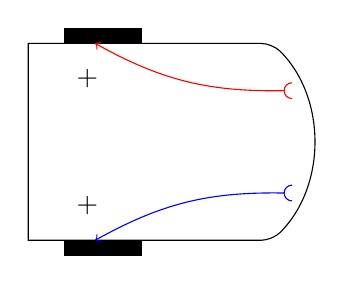
\begin{tikzpicture}[scale=.5]
% Draw big robot
\draw (-2.2cm,-2.5cm) to [rounded corners] (4cm,-2.5cm) to [rounded corners, bend right=45] (4cm,2.5cm) to (-2.2cm,2.5cm) to cycle;
\fill (-1.3cm,-2.5cm) rectangle +(2cm, -.4cm);
\fill (-1.3cm,2.5cm) rectangle +(2cm, .4cm);
\coordinate (right-wheel) at (-.5,-2.5);
\coordinate (left-wheel) at (-.5,2.5);
\node[below,xshift=-1mm,yshift=-2mm] at (left-wheel) {$+$};
\node[above,xshift=-1mm,yshift=2mm] at (right-wheel) {$+$};
% Left sensor and arrows
\coordinate (left-sensor) at (4.3,1.3);
\draw[red] (4.5, 1.5) arc[start angle=90, end angle=270, radius=.2cm];
\draw[->,red] (left-sensor) to [bend left=15] (left-wheel);
% Right sensor and arrows
\coordinate (right-sensor) at (4.3,-1.3);
\draw[blue] (4.5, -1.5) arc[start angle=270, end angle=90, radius=.2cm];
\draw[->,blue] (right-sensor) to [bend right=15] (right-wheel);
\end{tikzpicture}
}
\hspace{\fill}
\rightfigure[c]{
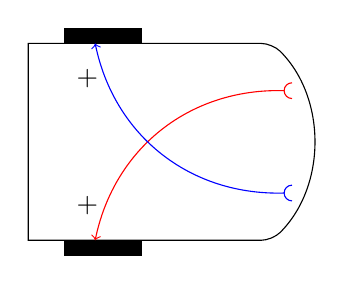
\begin{tikzpicture}[scale=.5]
% Draw big robot
\draw (-2.2cm,-2.5cm) to [rounded corners] (4cm,-2.5cm) to%
[rounded corners, bend right=45] (4cm,2.5cm) to (-2.2cm,2.5cm) to cycle;
\fill (-1.3cm,-2.5cm) rectangle +(2cm, -.4cm);
\fill (-1.3cm,2.5cm) rectangle +(2cm, .4cm);
\coordinate (right-wheel) at (-.5,-2.5);
\coordinate (left-wheel) at (-.5,2.5);
\node[below,xshift=-1mm,yshift=-2mm] at (left-wheel) {$+$};
\node[above,xshift=-1mm,yshift=2mm] at (right-wheel) {$+$};
% Left sensor and arrows
\coordinate (left-sensor) at (4.3,1.3);
\draw[red] (4.5, 1.5) arc[start angle=90, end angle=270, radius=.2cm];
\draw[->,red] (left-sensor) to [bend right=40] (right-wheel);
% Right sensor and arrows
\coordinate (right-sensor) at (4.3,-1.3);
\draw[blue] (4.5, -1.5) arc[start angle=270, end angle=90, radius=.2cm];
\draw[->,blue] (right-sensor) to [bend left=40] (left-wheel);
\end{tikzpicture}
}
\leftcaption{Coward vehicle\label{fig.coward}}
\rightcaption{Aggressive vehicle\label{fig.aggressive}}
\end{minipage}
\end{figure}

\begin{framed}
\act{Braitenberg's presentation of the vehicles}{brait-vehicles}
\begin{itemize}
\item Implement the \emph{coward} and \emph{aggressive} vehicles.
\item Use proximity sensors in place of Braitenberg's light sensors and the detection or non-detection of an object in place of stronger or weaker light sources.
\item The robots in Figs.~\ref{fig.loves}--\ref{fig.explorer} are the same as the robots in Figs.~\ref{fig.coward}--\ref{fig.aggressive}, respectively, except that the values of the sensors are negated (the $-$ signs on the connections): the more light detected, the slower the wheel will turn. Assume that there is a fixed bias applied to the motors so that the wheels turn forwards when no light source is detected.
\item Implement the robot in Fig.~\ref{fig.loves}. Why is it called \emph{loves}?
\item Implement the robot in Fig.~\ref{fig.explorer}. Why is it called \emph{explorer}?
\end{itemize}
\end{framed}


\begin{figure}
\subfigures
\begin{minipage}{\textwidth}
\leftfigure[c]{
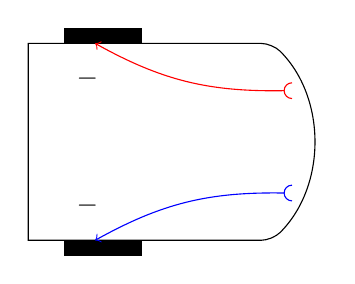
\begin{tikzpicture}[scale=.5]
% Draw big robot
\draw (-2.2cm,-2.5cm) to [rounded corners] (4cm,-2.5cm) to%
[rounded corners, bend right=45] (4cm,2.5cm) to (-2.2cm,2.5cm) to cycle;
\fill (-1.3cm,-2.5cm) rectangle +(2cm, -.4cm);
\fill (-1.3cm,2.5cm) rectangle +(2cm, .4cm);
\coordinate (right-wheel) at (-.5,-2.5);
\coordinate (left-wheel) at (-.5,2.5);
\node[below,xshift=-1mm,yshift=-2mm] at (left-wheel) {$-$};
\node[above,xshift=-1mm,yshift=2mm] at (right-wheel) {$-$};
% Left sensor and arrows
\coordinate (left-sensor) at (4.3,1.3);
\draw[red] (4.5, 1.5) arc[start angle=90, end angle=270, radius=.2cm];
\draw[->,red] (left-sensor) to [bend left=15] (left-wheel);
% Right sensor and arrows
\coordinate (right-sensor) at (4.3,-1.3);
\draw[blue] (4.5, -1.5) arc[start angle=270, end angle=90, radius=.2cm];
\draw[->,blue] (right-sensor) to [bend right=15] (right-wheel);
\end{tikzpicture}
}
\hspace{\fill}
\rightfigure[c]{
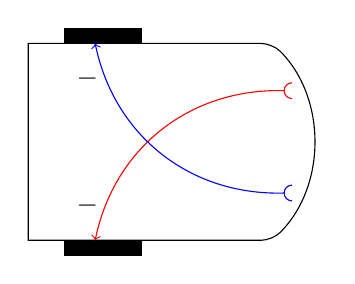
\begin{tikzpicture}[scale=.5]
% Draw big robot
\draw (-2.2cm,-2.5cm) to [rounded corners] (4cm,-2.5cm) to%
[rounded corners, bend right=45] (4cm,2.5cm) to (-2.2cm,2.5cm) to cycle;
\fill (-1.3cm,-2.5cm) rectangle +(2cm, -.4cm);
\fill (-1.3cm,2.5cm) rectangle +(2cm, .4cm);
\coordinate (right-wheel) at (-.5,-2.5);
\coordinate (left-wheel) at (-.5,2.5);
\node[below,xshift=-1mm,yshift=-2mm] at (left-wheel) {$-$};
\node[above,xshift=-1mm,yshift=2mm] at (right-wheel) {$-$};
% Left sensor and arrows
\coordinate (left-sensor) at (4.3,1.3);
\draw[red] (4.5, 1.5) arc[start angle=90, end angle=270, radius=.2cm];
\draw[->,red] (left-sensor) to [bend right=40] (right-wheel);
% Right sensor and arrows
\coordinate (right-sensor) at (4.3,-1.3);
\draw[blue] (4.5, -1.5) arc[start angle=270, end angle=90, radius=.2cm];
\draw[->,blue] (right-sensor) to [bend left=40] (left-wheel);
\end{tikzpicture}
}
\leftcaption{Loves vehicle\label{fig.loves}}
\rightcaption{Explorer vehicle\label{fig.explorer}}
\end{minipage}
\end{figure}

\section{Summary}

A robot exhibits reactive behavior when its actions depend only upon the current values returned by its sensors. This chapter presented two families of reactive behavior. Braitenberg vehicles implement reactive behavior by changing the setting of the motors in response to the events of proximity sensors detecting or not detecting an object at some position relative to the robot. The vehicles demonstrate that complex behavior can result from relatively simple reactive algorithms.

Line following is a fundamental task in robotics. Because of uncertainties of the robot's motion and its environment, robots use landmarks such as lines to ensure that they move to their intended destination. Line following is a reactive behavior because the robot modifies its behavior in response to values returned by the ground sensors. We have given three configurations for the robot and the line, and developed algorithms for each case. The performance of the algorithms depends on the sensor thresholds and the motor speeds, which must be determined by experimentation in order to ensure that the robot moves rapidly while remaining robust to changes in the environment.

\section{Further reading}

Braitenberg's book \cite{valentino} is interesting because he writes from the perspective of a neuroscientist. The book describes vehicles using imagined technology, but they are nevertheless thought-provoking. The Braitenberg vehicles described here are adapted from the hardware implementations described in \cite{creatures}. An implementation of the Braitenberg vehicles in Scratch by the first author can be found at:\par\noindent\url{https://scratch.mit.edu/studios/1452106}.

\bibliographystyle{spmpsci}
\bibliography{er}
